\chapter{Introduction}

%Provide a short summary of the whole PhD thesis:
% -Introduction to QC & CQED
% -Building Blocks of Superconducting Quantum Processors
% -Realization of a 2-Transmon QP
% -Tune-Up & Characterization of the Universal 2-Qubit Gate
% -Grover's Algorithm: Introduction & Background
% -Implementation on the 2-Qubit Processor
% -Design of a Scalable QC Architecture

\section{Quantum Computing \& Circuit Quantum Electrodynamics}

\begin{figure}
	\centering
		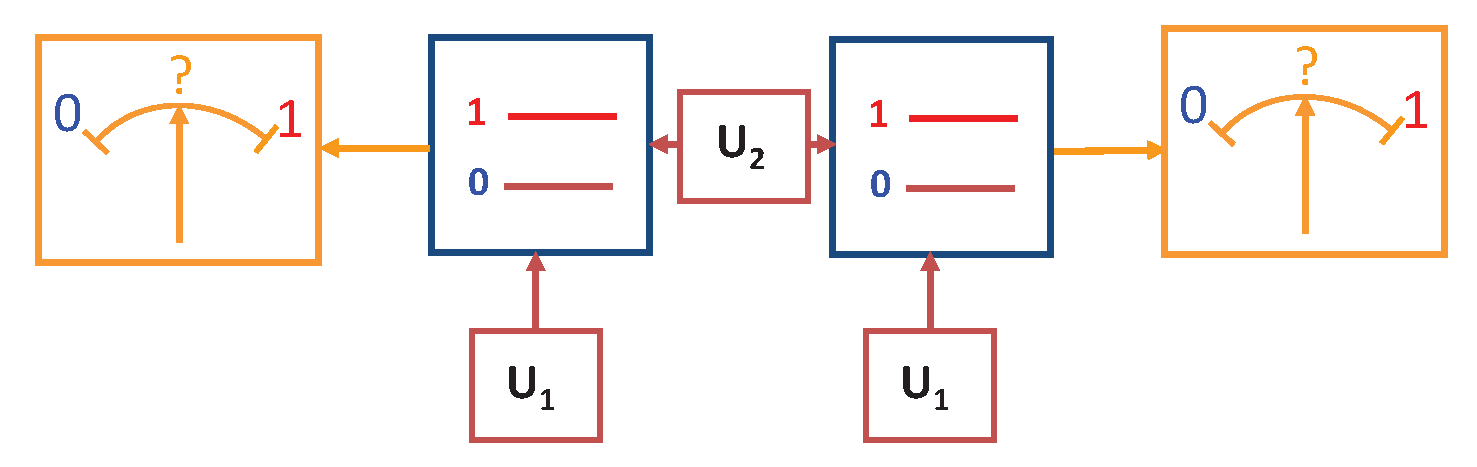
\includegraphics[width=1.\textwidth]{./material/papers/grover/submission1/Fig1}
	\label{fig:Grover1}
	\caption{The blueprint of a 2 qubit quantum processor. Shown a two qubits which can be manipulated individually ($U_1$) and which possess a universal two-qubit gate $U_2$. Each of the qubits can be read out individually.}
\end{figure}

This thesis presents experiments performed on on superconducting 2-Qubit quantum processor. The main goal of this work was to demonstrate a possible quantum computing architecture using superconducting qubits that follows the canonical blueprint of a 2-qubit quantum processor as formulated by \cite{divincenzo_physical_2000} and as shown in fig. \ref{fig:Grover1}. In this respect, a universal quantum computer is a register of quantum bits -- or qubits -- on which one can perform universal 1- and 2-qubit quantum gates. In addition, one can read out the state of each qubit individually and with high fidelity and reset the qubit register to a well-defined product state.

Implementing this allegedly simple list of requirements in a system of superconducting qubits has been a major research challenge during the last decade. The first demonstration of coherent quantum-mechanical dynamics in a superconducting structure by \cite{nakamura_coherent_1999} sparked a broad research field about superconducting quantum bits. In the years following Nakamura's discovery, several types of superconducting qubits were proposed and realized, using the superconducting phase \citep{martinis_energy-level_1985,martinis_rabi_2002} across a Josephson junction or the magnetic flux \citep{mooij_josephson_1999,chiorescu_coherent_2003} in a superconducting ring as the dominant quantum variable. Another milestone was the development of the so called {\it Quantronium} qubit \citep{vion_manipulating_2002}, which showed for the first time a coherence time larger than 1 $\mu s$ by using an intermediate regime between charge and phase qubits and operating the device at a sweetspot. This also made it possible to perform -- for the first time -- robust, high fidelity single-qubit operations with a superconducting qubit. In 2004, the development of a new type of qubit, the so called {\it Transmon} \citep{wallraff_strong_2004} drastically improved the quality of superconducting charge qubits by operating them deep in the phase regime and by embedding them in superconducting coplanar waveguide resonators, which allows for an easy and robust readout and yields a high qubit lifetime. Within this approach, quantum gates and algorithms with up to four qubits have been implemented, demonstrating multi-qubit entanglement \citep{dicarlo_preparation_2010} and simple quantum algorithms \citep{dicarlo_demonstration_2009}.

In parallel to this, the development of quantum-limited amplifiers based on non-linear superconducting resonators by \cite{siddiqi_rf-driven_2004} complemented the CQED architecture by providing a fast and high-fidelity readout scheme for Transmon qubits \citep{siddiqi_dispersive_2006,mallet_single-shot_2009} and for the amplification of quantum signals in general. This opened up the road to the direct observation of quantum jumps in superconducting qubits \citep{vijay_observation_2011} and even for implementing simple forms of quantum feedback. \todo{Add reference to quantum feedback paper as soon as it appears}

Another important recent breakthrough is the development of a qubit architecture using three-dimensional superconducting cavitities instead of one-dimensional coplanar waveguide resonators in the CQED approach \cite{paik_observation_2011}. Producing an increase in qubit lifetime of one order of magnitude, this technique opened the road to more complex quantum feedback and error correction experiments.

This work wants to fit in this global picture by complementing the CQED approach with a single-shot, individual qubit readout. Such a readout is absolutely necessary when pursuing the long-term goal of a superconducting quantum computer but -up to now- was just not provided by ``classical'' CQED.

\section{Building a Superconducting Quantum Processor}

To build a superconducting quantum processor, several ``ingredients'' have to be realized. The following section will therefore discuss the process of implementing the different elements of such a processor.

\subsection{Building Blocks}

According to \cite{divincenzo_physical_2000}, a quantum processor need to fulfill the following criteria:

\begin{itemize}
\item Well-defined qubits.
\item A way to initialize the qubits to a well-defined state.
\item High-fidelity readout of individual qubits.
\item A universal set of 1- and 2-qubit gates.
\end{itemize}

The most basic system that can implement all of these requirements is a 2-qubit processor, which we therefore used in this work as a ``model'' quantum processor which -- to varying degrees -- demonstrates all of the above criteria.

\subsection{Processor design}

\begin{figure}
	\centering
		\includegraphics[width=1.\textwidth]{./material/papers/grover/figures/2_qubit_processor_schematic}
	\label{fig:two_qubit_processor_schematic}
	\caption{Circuit schematics of the two-qubit processor realized in this work, showing the two qubits in green, the qubit readouts in blue and the fast flux lines in red. Each qubit is embedded in its own nonlinear readout resonator and can be driven and read out through an individual microwave line. The simultaneous single-shot readout of the two qubits produces measurement outcomes in the basis $x \in \{00,01,10,11\}$.}
\end{figure}

The quantum processor implemented in this work is shown in fig. (\ref{fig:two_qubit_processor_schematic}) consists of two superconducting quantum bits of the Transmon-type, each equipped with its own drive and readout circuit consisting of a nonlinear coplanar-waveguide resonator used as a Josephson bifurcation amplifier (JBA). The qubit frequencies can be controlled individually by two fast flux lines. The coupling between the qubits is realized through a fixed capacitive coupling.

In the following sections we will discuss the details of each element of this processor.

\subsection{Simultaneous Single-Shot Qubit Readout}

To read out the state of each qubit is done by using a so-called Josephson bifurcation amplifier \citep{siddiqi_dispersive_2006,mallet_single-shot_2009}. This readout works by capacitively coupling the qubit to a coplanar waveguide resonator which is rendered nonlinear by adding a Josephson junction at the center of the resonator. This nonlinear resonator can exhibit bistable behaviour for certain drive parameters, which we can use to map the state of the qubit to one of the bistable states of the resonator, thus obtaining a high-fidelity, single-shot readout of the qubit. In contrast to other CQED architectures, each of the two qubits of our processor possesses its own JBA readout, which follows the diVincenzo criteria by allowing a simultaneous measurement of the state of the whole qubit register. The fidelity attained with a JBA readout can be as high as 93 \% \citep{mallet_single-shot_2009}, but due to design contraints was usually around 85 \% for the quantum processor realized here.

\subsection{Two-Qubit Quantum Operations}

\begin{figure}
	\centering
		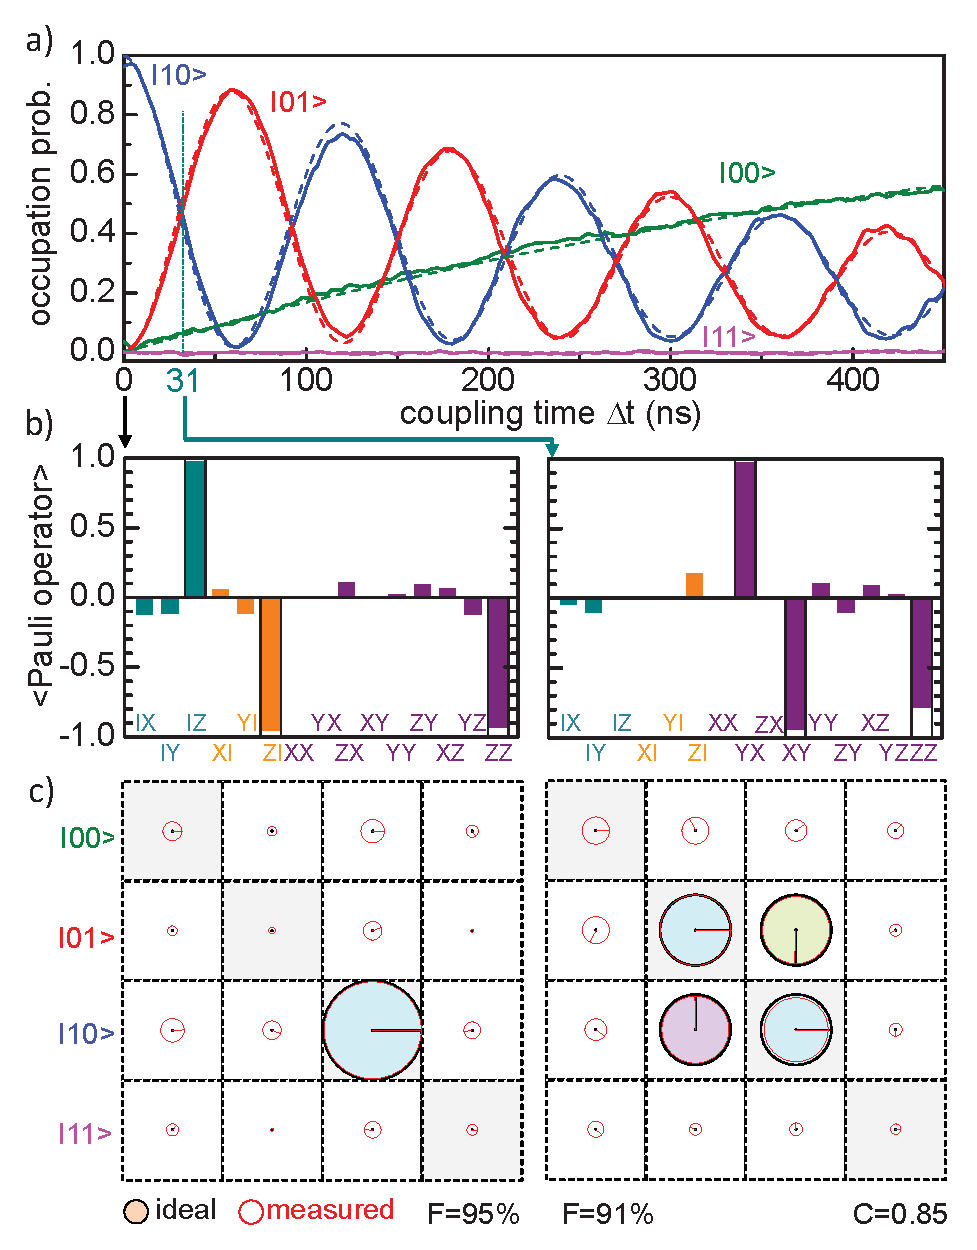
\includegraphics[width=0.9\textwidth]{./material/papers/iswap/submission1/Dewes_Figure2}
	\label{fig:iSwap2}
	\caption{An experiment showing the creation of entanglement between the two qubits and the realization of the universal $\sqrt{i\mathrm{SWAP}}$ quantum gate. The qubits start out seperated in frequency and are initialized to the state $\ket{10}$. Afterwards, the qubit frequencies are non-adiabatically tuned into resonance and held there for a well-defined time $\Delta t$. When measuring the $\sigma_z^1 \otimes \sigma_z^2$ operator of the system, an energy exchange between the states $\ket{01}$ and $\ket{10}$ can be observed. The reconstruction of the full quantum state of the system after an interaction time of $\Delta t = 31 \; \mathrm{ns} $ by quantum state tomography shows entanglement between the qubits. By adding compensating $\sigma_z^{1,2}$ pulses after the application of the entanglement gate one can implement the $\sqrt{i\mathrm{SWAP}}$ gate.}
\end{figure}

The fixed coupling between the two qubits of our processor provides a $\sigma_{xx}$-type coupling of the qubits. This coupling is effective only when the qubit frequencies are near-resonance and can thus be switched on and off by changing the qubit frequencies. In the processor realized here, the effective qubit-qubit coupling  of the qubits was of the order of $2g = 8.2 \; \mathrm{MHz}$.\todo{Check if this is really $2g$!}

Using the $\sigma_x$ coupling of the qubits, we can implement the so called $\sqrt{i\mathrm{SWAP}}$ gate, which is a universal 2-qubit quantum gate and has the unitary representation

\begin{equation}
	\sqrt{i\mathrm{SWAP}}  =  \left( \begin{array}{cccc} 1/\sqrt{2} & 0 & 0 & 0 \\ 0 & 1/\sqrt{2} & i/\sqrt{2} & 0 \\ 0 & i/\sqrt{2} & 1/\sqrt{2} & 0 \\ 0 & 0 & 0 & 1/\sqrt{2} \end{array} \right) \label{eq:sqrt_iswap_gate}
\end{equation}

This gate is realized by starting with the two qubits seperated in frequency such that the coupling between them is negligable. After initializing the qubits to a given state, the qubit frequencies are tuned in resonance non-adiabatically by changed the magnetic flux in on of the two qubit loops. Holding the qubits at resonance for a well-defined time $\Delta t$ and seperating them non-adiabatically afterwards can produce an entangled qubit state, as shown in fig. (\ref{fig:iSwap2}). 

With the realized quantum processor we attain a gate fidelity of 90 \% for this quantum gate, which is good enough to demonstrate simple quantum algorithms with the system.

\subsection{Running a Quantum Algorithm}

The demonstration of quantum speed-up is an important benchmark for any prospective quantum processor. In this work, we implemented a compiled version of Grover's search algorithm \citep{Grover_Quantum_1997}. Our version of the algorithm works in the basis of two qubits $x_i \in \{\ket{00},\ket{01},\ket{10},\ket{11}\}$and in theory can distinguish between four different ``oracle functions'' $f(x)$ which mark a given state $x_j$ and leave the other states unchanged. Since the algorithm requires only one evaluation of the function $f(x)$ to determine which state has been marked it is 50 \% faster than any conceivable algorithm using classical compuation \comment{discuss again if this should be 25 \% or 50 \%}. In this work, the single-run fidelity of the algorithm ranges between 52 and 67 \%, depending on the marked state $x_j$, which clearly demonstrates quantum speed-up in this system, although only on a quite artificial and practically irrelevant problem.

\section{Scaling Up To Multiple Qubits}

After having demonstrated the different building blocks of a superconducting, Transmon-based quantum processor it remains to be shown that larger-scale quantum-computing beyond two qubits is possible with this system. This work therefore pursued the realization of a more scalable qubit architecture using systems of up to six qubits coupled through a so-called ``quantum bus'' \citep{majer_coupling_2007}. The details of this novel architecture are discussed in the following sections.

\subsection{Multi-Qubit Quantum Computing Architecture}

The approach for scalable quantum computing with superconducting qubits pursued in this work consists of a system of many individual Transmon qubits equipped with individual JBA-based readouts, a multiplexed drive and readout circuit and a fixed qubit-qubit coupling mediated through a high-Q CPW resonator. As before, each qubit possesses a fluxline for fast frequency control. The readout and drive signals are send to all the qubits in parallel through a multiplexed 50 $\Omega$ transmission line. In this approach, the frequencies of the JBA readouts have to be chosen such that driving individual readouts at a given frequency does not induce crosstalk or spurious coupling to other readout resonators. Also, the transition frequencies of all qubits have to be chosen such that it becomes possible to individually address each of them without inducing transitions in the other qubit states.

\subsection{Implementation}

\begin{figure}
	\centering
		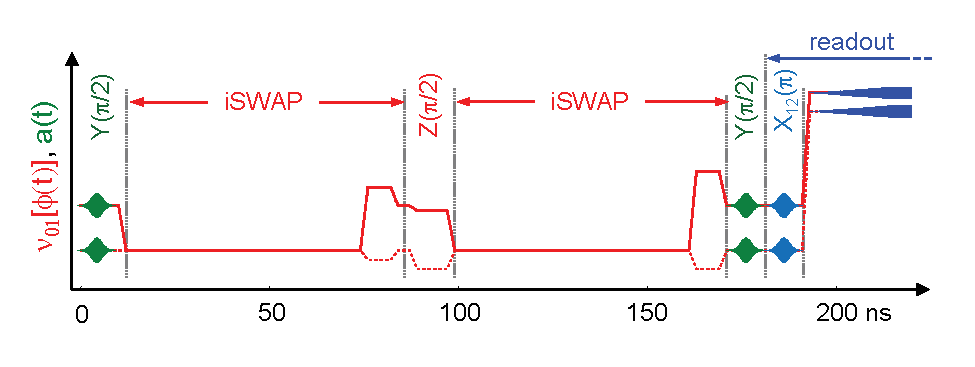
\includegraphics[width=1.\textwidth]{./material/papers/grover/figures/grover_algorithm_pulse_sequence}
	\label{fig:Grover3}
	\caption{The pulse sequence used in realizing Grover's quantum search algorithm. First, a $Y_{\pi/2}$ pulse is applied to each qubit to produce the fully superposed state $1/2(\ket{00}+\ket{01}+\ket{10}+\ket{11})$. Then, an $i\mathrm{SWAP}$ gate is applied, followed by a $Z_{\pm \pi /2}$ gate on each qubit, which corrsponds to the application of the oracle function. The resulting state is then analyzed using another $i\mathrm{SWAP}$ gate and two $Y_{\pi/2}$ gates to extract the state which has been marked by the oracle function. Optionally, a $Y^{12}_{\pi}$ pulse is used on each qubit to increase the readout fidelity.}
\end{figure}


%2 Qubit Paper Figures

\begin{figure}
	\centering
%		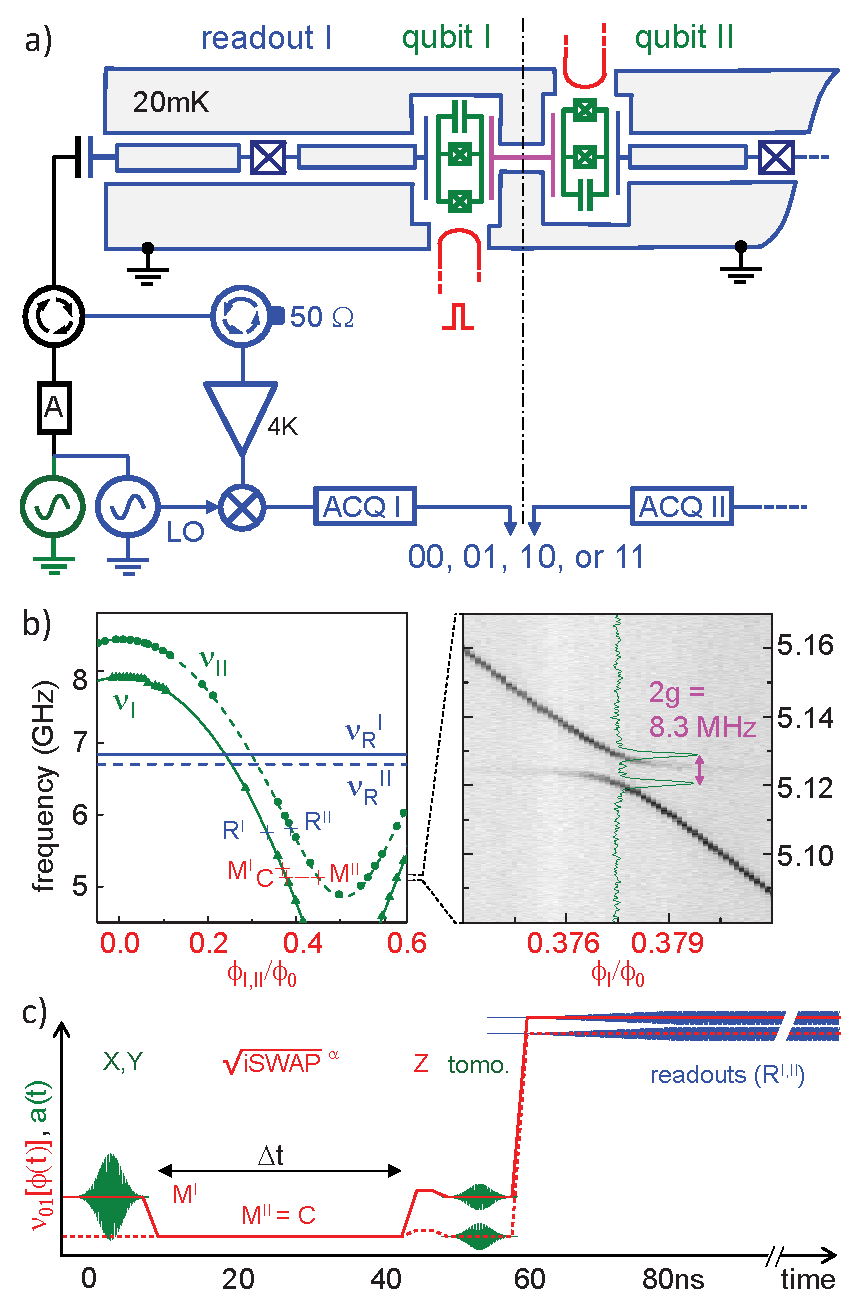
\includegraphics[width=1.\textwidth]{./material/papers/iswap/submission1/Dewes_Figure1}
	\label{fig:iSwap1}
	\caption{}
\end{figure}

\begin{figure}
	\centering
		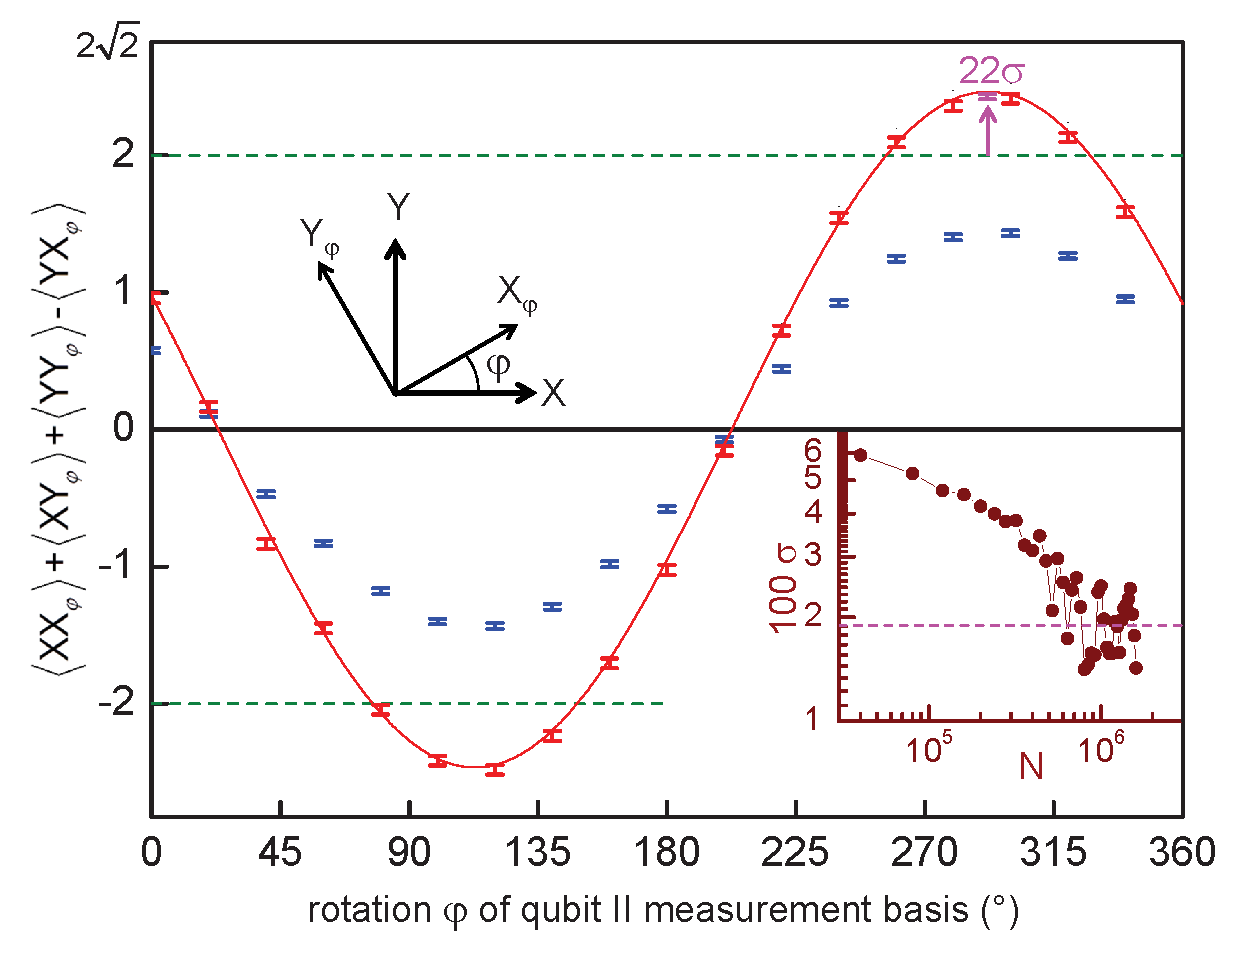
\includegraphics[width=1.\textwidth]{./material/papers/iswap/submission1/Dewes_Figure3}
	\label{fig:iSwap3}
	\caption{}
\end{figure}

\begin{figure}
	\centering
		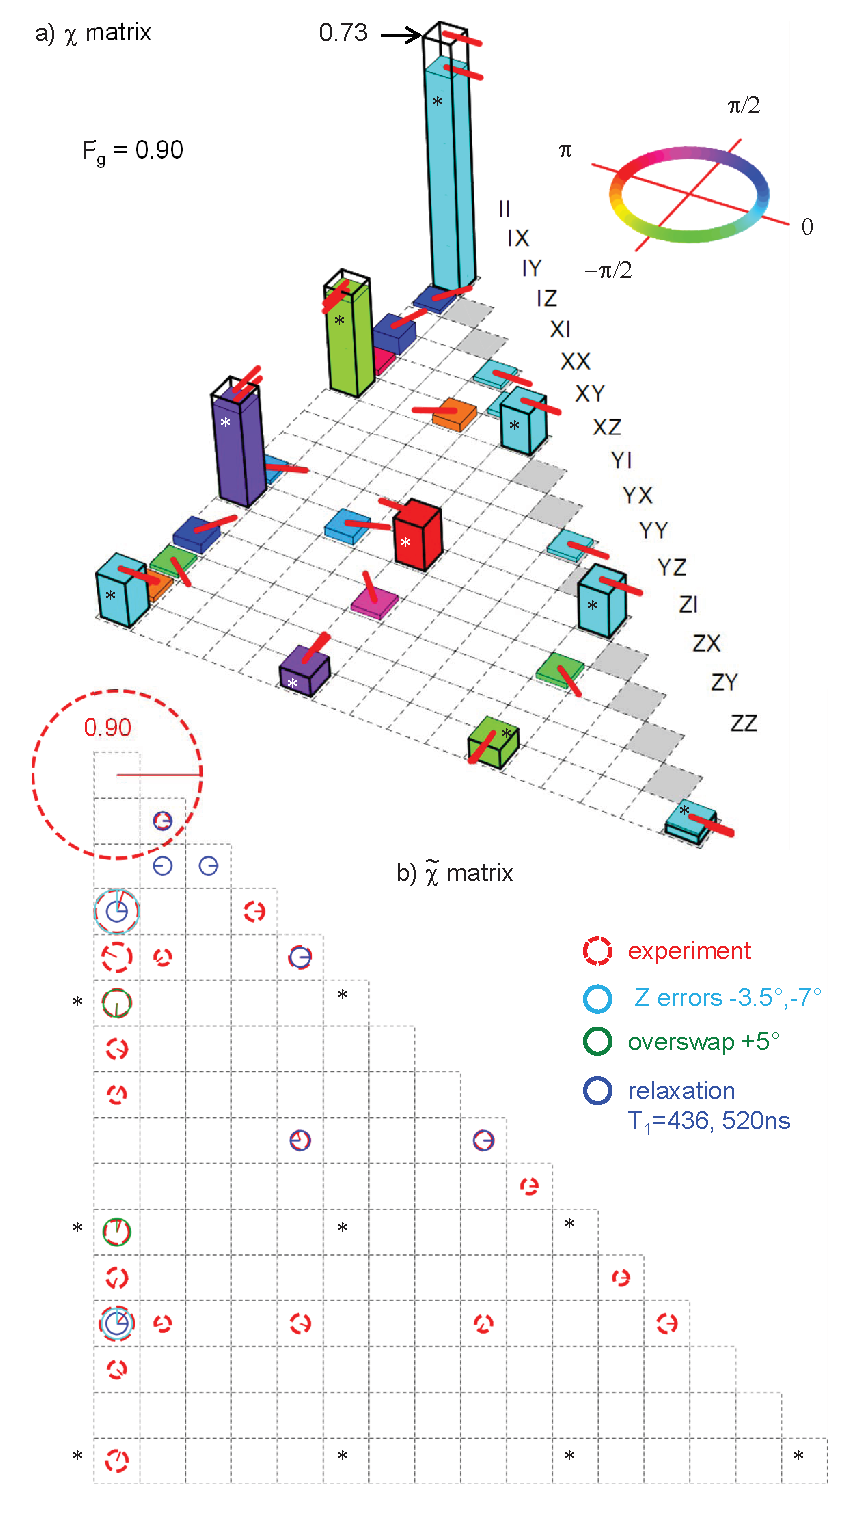
\includegraphics[width=1.\textwidth]{./material/papers/iswap/submission1/Dewes_Figure4}
	\label{fig:iSwap4}
	\caption{}
\end{figure}
